\documentclass[11pt,jaso]{pnumasterh}
%\documentclass[11pt,a4paper]{pnumasterh}
\usepackage[ruled,linesnumbered,vlined]{algorithm2e}
\usepackage{amsmath,amssymb,amsfonts}
\usepackage{color,fancyvrb,alltt}
\usepackage{listings, chngcntr}
\usepackage{colortbl, booktabs}
\usepackage[subfigure]{tocloft}
\usepackage{threeparttable}
\usepackage{verbatimbox}
\usepackage{indentfirst}
\usepackage{algorithmic}
\usepackage{subfigure}
\usepackage{longtable}
\usepackage{textcomp}
\usepackage{floatrow}
\usepackage{graphicx}
\usepackage{setspace}
\usepackage{multirow}
\usepackage{csquotes}
\usepackage{setspace}
\usepackage{fancyvrb}
\usepackage{geometry}
\usepackage{sidecap}
\usepackage{caption}
\usepackage{courier}
\usepackage{amsmath}
\usepackage{courier}
\usepackage{amsmath}
\usepackage{amssymb}
\usepackage{amsthm}
\usepackage{epsfig}
\usepackage{hhline}
\usepackage{kotex}
\usepackage{float}
\usepackage{array}     
\usepackage{color}
\usepackage{xfrac}
\usepackage{url}

\definecolor{mygreen}{rgb}{0   , 0.6, 0   }
\definecolor{mygray }{rgb}{0.5 , 0.5, 0.5 }
\definecolor{mymauve}{rgb}{0.58, 0  , 0.82}
\renewcommand\lstlistingname{Algorithm}
\floatsetup[table]{capposition=top}

\newcolumntype{C}[1]{>{\centering\arraybackslash}m{#1}}
\definecolor{Gray}{gray}{0.9}

\urlstyle{same}
\definecolor{red}{rgb}{1, 0, 0}

\floatstyle{ruled}
\newfloat{algorithm}{htp}{loa}
\floatname{algorithm}{a}

\newfloat{mybox}{htp}{lob}
\newcommand{\DRule}{\rule[4pt]{\linewidth}{0.5mm}}
\newcommand{\SRule}{\rule[4pt]{\linewidth}{0.1mm}}

\newcommand{\argmax}{\operatornamewithlimits{argmax}}
\newtheorem{definition}{정의}[subsection]
\newtheorem{example}{예제}[subsection]
\newtheorem{theorem}{정리}[subsection]

\newcommand{\abs}[1]{\lvert #1 \rvert}
\newenvironment{smalltt}{\scriptsize\begin{alltt}}{\end{alltt}\normalsize}

\DeclareCaptionFormat{mylst}{\hrule#1#2#3}

\newenvironment{CVerbatim}
	{\singlespacing\center\BVerbatim}
	{\endBVerbatim\endcenter}

\htitle{\huge \vspace{-5mm} Comparative Analysis of Cross-Platform and Native Mobile App Development Approaches \vspace{-5mm}}
\title{Comparative Analysis of Cross-Platform and Native Mobile App Development Approaches}
\hauthor{ Ibrokhimov Sardorbek Rustam Ugli}
\author{Ibrokhimov Sardorbek Rustam Ugli}

\etitle{\huge 교차 플랫폼 및 네이티브 모바일 앱 개발 접근 방식의 비교 분석 } 
\eauthor{이브로키모브 사도르벡}
\edept{정 보 융 합 공 학 과} 
\hdept{Department of Information Convergence Engineering}
\huniv{Pusan National University} 
\euniv{부 산 대 학 교}

\hdegree{Thesis for the degree of Master of Science} \degree{Thesis for the degree of Master of Science}

\htutor{Gyun Woo}


\principaladvisor{Hwan-Gue Cho} \subadva{Heung-Seok Chae}
\subadvb{Gyun Woo}

\graddate{August 2024}

\submitdate{May 31, 2024}

\begin{document}
\maketitle 
\pagestyle{empty}

\newpage
\pagestyle{plain} \pagenumbering{roman}

\setlength\cftsecnumwidth{2.3em}

\tableofcontents
\newpage
\listoffigures 
\newpage
\listoftables 


\newpage
\thispagestyle{empty}
\begin{center}
    \vskip 3.5cm
    {\Large{Comparative Analysis of Cross-Platform and Native Mobile App Development Approaches}} \\
    \vskip 15mm
    {\large{Ibrokhimov Sardorbek Rustam Ugli}} \\
    \vskip 10mm
    {Department of Information Convergence Engineering} \\
    {The Graduate School} \\
    {Pusan National University} \\
    \vskip 15mm
    {\large{Abstract}}\\
    \vskip 10 mm
\end{center}

Though lots of approaches to developing mobile apps have been suggested up to now, developers have difficulties selecting the right one. This study compares native and cross-platform application development approaches, particularly focusing on the shift in preference from Java to Kotlin and the increasing use of Flutter. This research offers practical insights into factors influencing developers’ choice of programming languages and frameworks in mobile application development by creating identical applications using Java, Kotlin, and Dart (Flutter). Furthermore, this study explores the best practices for development by examining the quality of code in 45 open-source GitHub repositories. The study evaluates LOC and code smells using semi-automated SonarQube assessments to determine the effects of selecting a specific language or framework on code maintainability and development efficiency. Preliminary findings show differences in the quality of the code produced by the two approaches, offering developers useful information on how to best optimize language and framework selection to reduce code smells and improve project maintainability.    
\newpage
\pagenumbering{arabic}

\section{Introduction}
\subsection{The Rise of Mobile Applications }
Mobile applications have become integral to daily life globally, revolutionizing various sectors such as healthcare, education, finance, and entertainment. The rise of mobile applications has significantly impacted society, leading to increased dependence on mobile technologies. Integrating information and communication technologies (ICTs) like mobile phones and the Internet with financial services has given rise to new forms of digital finance, including mobile payments, online credit, and intelligent investment advice \cite{li2022impact}. This integration has transformed financial services and facilitated access to formal financial services for underserved populations, such as smallholder farmers \cite{omar2022predictors}.
\par
The rapid growth of the mobile app market is evident in the increasing adoption of mobile payment systems. Mobile payment systems have increased employment and income for family members, particularly benefiting low-income and rural households \cite{wang2020mobile}. Moreover, the development of financial innovations like mobile payments and AI-based credit scoring systems has immense potential to increase financial inclusion, enabling the unbanked population to participate actively in financial markets \cite{rybakovas2022financial}.
\par
In addition to finance, mobile applications have also played a crucial role in healthcare. Mobile smartphone applications provide a unique platform to promote the utilization of evidence-based skills, especially in areas like substance use treatment \cite{dahne2015smartphone}. Furthermore, the education sector has witnessed a transformation with the increasing use of mobile applications. The study indicates that mobile banking, a mobile application, has provided smallholder farmers access to formal financial services like deposits and loans, which previously needed to be improved \cite{omar2022predictors}.
\par
Entertainment is another sector significantly impacted by mobile applications. Note that mobile phones, through various entertainment apps, compete for limited attention with social networks, videos, games, and other types of entertainment \cite{zhang2023entertainment}. This competition for attention underscores the widespread use and popularity of entertainment apps on mobile devices.
\begin{figure}[htbp]
    \centering
    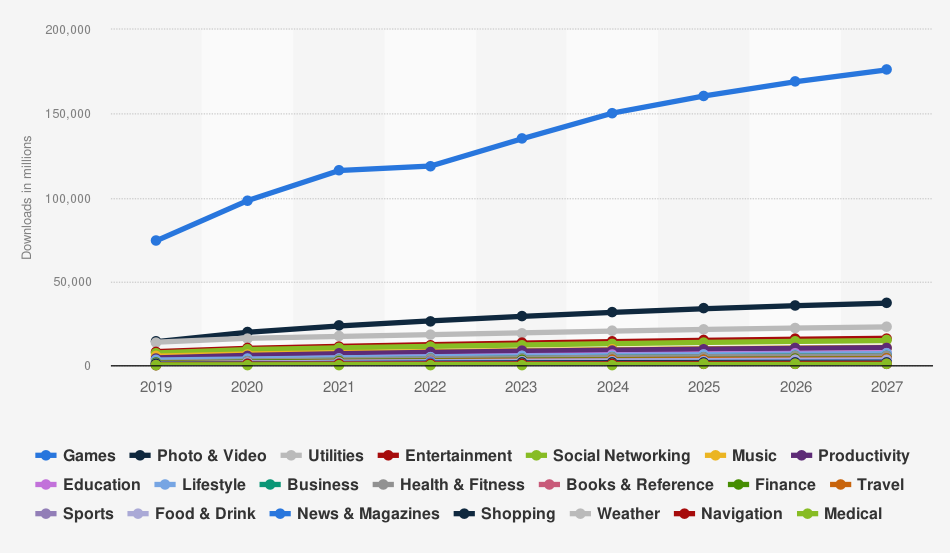
\includegraphics[scale = 0.45]{img/num_of_downloads.png}
    \caption{Number of mobile app downloads worldwide from 2019 to 2027, by segment(in million downloads) \cite{statista2023}}
    \label{fig:num_of_downloads}
\end{figure}
\par
The Figure \ref*{fig:num_of_downloads} clearly illustrates a continuous and significant growth in mobile application downloads across all sectors, with projections reaching up to 176.1 billion downloads in the Games segment by 2027. This trend, consistent throughout the forecast period from 2019 to 2027, emphasizes the expanding role and importance of mobile applications in daily life and various industries.
\par
The statistics and trends in mobile application usage globally reflect a trajectory of growth and innovation. The increasing reliance on mobile technologies across sectors underscores the transformative impact of mobile applications on society, paving the way for enhanced accessibility, efficiency, and convenience in various aspects of daily life. 
\subsection{Evolution of Mobile Development Approaches}
The evolution of mobile app development has seen significant advancements from early platforms to the modern ecosystems of Android and iOS. Initially, Java dominated Android development, offering a robust and versatile language for creating mobile applications. However, the introduction of Kotlin by JetBrains marked a pivotal moment in Android development. Kotlin, with its concise syntax, enhanced safety features, and seamless interoperability with Java, quickly gained popularity among developers. Google recognized the potential of Kotlin and endorsed it as a preferred language for Android app development, leading to widespread adoption within the Android community \cite{zhang2023entertainment}.
\par
Moreover, the emergence of cross-platform frameworks has revolutionized mobile app development by enabling developers to write code once and deploy it across multiple platforms. Flutter, developed by Google, has gained prominence among these frameworks for its efficiency and flexibility in building high-quality native interfaces. Flutter allows for fast development, expressive UIs, and native performance, making it popular for developers aiming to create visually appealing and responsive applications.
\par
Adopting Kotlin and Flutter signifies a shift towards more efficient and streamlined mobile app development practices. Kotlin's modern features and seamless integration with existing Java codebases have simplified the development process. At the same time, Flutter's cross-platform capabilities have empowered developers to create visually rich and performant applications across different operating systems. These advancements highlight the continuous evolution of mobile development approaches, emphasizing the importance of innovation and adaptability in the ever-changing landscape of mobile technology.
\subsection{Evolution of Mobile Development Approaches}
Choosing between native development and cross-platform frameworks is a strategic decision that goes beyond technical considerations and impacts the success of a mobile application. Native development offers optimized performance and better access to device-specific features, ensuring high user satisfaction. On the other hand, cross-platform frameworks provide advantages such as faster rollout and cost-effectiveness. The decision between these approaches has implications for app performance, maintainability, and overall user experience, making selecting the appropriate development approach crucial.
\par
Native development, often associated with languages like Java for Android and Swift for iOS, allows developers to leverage platform-specific features and functionalities, resulting in high-performance applications tailored to each operating system. However, the development time and cost for native apps can be higher due to the need to write separate codebases for different platforms.
\par
In contrast, cross-platform frameworks like Flutter, React Native, and Xamarin enable developers to write code once and deploy it across multiple platforms, reducing development time and costs. While cross-platform development offers advantages in terms of efficiency and cost-effectiveness, there may be trade-offs in terms of performance optimization and access to certain platform-specific features.
\par
The study emphasizes the importance of well-defined technical requirements and specifications in selecting a cross-platform framework or development approach. Specific cross-platform frameworks can perform equally or even better than native in particular metrics, highlighting the need for a deliberate and informed decision-making process \cite{biorn2020empirical}.
\par
Ultimately, the choice between native development and cross-platform frameworks should align with the mobile application’s project requirements, budget constraints, and long-term goals. Understanding the implications of each approach on app performance, maintainability, and user satisfaction is essential for making an informed decision that maximizes the mobile application's success.
\subsection{Comparative Analysis: Java, Kotlin, and Flutter }
Java and Kotlin have been long-standing choices for native Android app development, with Java being the traditional standard and Kotlin emerging as a modern alternative. Java, known for its robustness and extensive ecosystem, has been widely used for Android development \cite{wasilewski2021comparison}. On the other hand, Kotlin, being interoperable with Java, offers a more concise syntax and additional safety features, enhancing code readability and reducing bugs \cite{ardito2020effectiveness}. The transition from Java to Kotlin has been notable, with Google endorsing Kotlin as the preferred language for Android app development \cite{coppola2019characterizing}.
\par
In contrast, Flutter, utilizing Dart, has gained attention for its cross-platform capabilities. It offers a single codebase for both Android and iOS platforms. This approach dramatically simplifies development and reduces maintenance costs \cite{prasetia2023development}. Flutter has been recognized as a framework that streamlines the development of cross-platform applications, providing efficiency and cost-effectiveness \cite{Meiller_2022}.
\par
The comparative analysis of Java, Kotlin, and Flutter reveals distinct advantages and challenges associated with each technology. Java and Kotlin excel in native Android development, with Kotlin offering modern features and improved safety. On the other hand, Flutter stands out for its cross-platform capabilities, enabling developers to create applications for multiple platforms with a single codebase. Understanding the strengths and limitations of each technology is essential for making informed decisions in mobile app development.
\subsection{Critical Role of Code Quality}
The quality of code is a vital component of software development, as it has a significant impact on the performance, scalability, and maintainability of applications. Key indicators of code quality include identifying code smells, which are patterns in the code that may indicate potential issues, and assessing the overall complexity of the codebase. Although code smells may not immediately affect the program's functionality, they can increase the risk of bugs or failures down the line and make maintenance more complex. Thus, it is critical to evaluate and address these smells to ensure the long-term quality and sustainability of software applications, as noted by Banker et al. \cite{banker1998software}.
\par
In software development, code quality is closely tied to developers' skills and capabilities. Research has shown that content software developers are more productive and effective in problem-solving. Psychological measurements in empirical software engineering have emphasized the significance of factors such as high analytical problem-solving skills and creativity in the software construction process, highlighting the role of developer well-being in software quality and productivity \cite{graziotin2014happy}.
\par
Efforts to enhance software quality often involve methodologies like the Capability Maturity Model (CMM), which aims to improve software development processes to deliver high-quality software within budget and planned cycle time. Adopting structured approaches like CMM can result in improved software quality, reduced defects, and increased efficiency in the software development lifecycle \cite{agrawal2007software}.
\par
Analyzing code quality across different programming languages and frameworks, such as Java, Kotlin, and Flutter, can offer valuable insights into the impact of development choices on software quality. Leveraging tools like SonarQube for evaluating and comparing code quality metrics can provide a quantitative basis for assessing the effectiveness of development practices and identifying areas for improvement. Developers can enhance software applications' overall quality and reliability by systematically analyzing code quality indicators and addressing issues such as code smells and complexity, improving user experiences and long-term success \cite{graziotin2018happens}.
\subsection{Research Gap}
Despite the critical role of mobile applications in various sectors and the rapid evolution of development technologies, there remains a significant gap in empirical research regarding the comparative analysis of mobile development approaches, particularly regarding their impact on code quality. Most existing studies focus on individual aspects of development, such as usability, performance, or developer preferences. Still, few comprehensively evaluate how different programming languages and frameworks—like Java, Kotlin, and Flutter—affect code's overall quality and maintainability.
\par
Current literature extensively discusses the features and benefits of Kotlin and Flutter, noting their potential to streamline the development process and enhance code safety and maintainability. However, more systematic empirical studies need to quantify the impact of these modern languages and frameworks on code quality in real-world development scenarios. This includes a detailed analysis of code smells, which are subtle indicators of potential future problems or technical debt that might not currently affect an application's functionality but could lead to significant maintenance challenges.
\par
Furthermore, while tools like SonarQube offer capabilities to assess and compare code quality metrics across different environments, the practical application of these tools in comparative studies must be extensively documented in academic research. Studies that not only use these tools to gather data but also critically analyze this data to provide actionable insights into how specific characteristics of Java, Kotlin, and Flutter influence the maintainability, scalability, and efficiency of the development process are needed.
\par
This research aims to fill these gaps by conducting a rigorous comparative analysis of mobile applications developed in Java, Kotlin, and Flutter. It will evaluate various code quality metrics, such as the prevalence and severity of code smells and the overall complexity of the codebases, to determine the tangible impacts of choosing one technology over another. This study will provide empirical evidence to guide developers in selecting the most suitable programming language or framework for their projects based on quantifiable code quality and maintainability measures.
\par
By addressing this research gap, the study will contribute valuable insights to the field of software engineering, particularly mobile app development. It will enhance understanding of the practical implications of development tool choices on long-term application success and sustainability.
\subsection{Study Objectives and Research Questions}
The overarching objective of this thesis is to conduct a thorough empirical analysis to compare the impact of different mobile development approaches—specifically Java, Kotlin, and Flutter—on the quality and maintainability of mobile applications. This research is driven by the need to provide developers and stakeholders with data-driven insights that can guide their decisions regarding which development technologies to adopt, depending on specific project requirements and goals. 
\par
The choice of focusing on these specific technologies is substantiated by their prevalent use and perceived benefits within the development community. According to a 2022 developer survey, Flutter has emerged as the most popular cross-platform mobile framework. The survey reports that 46 percent of software developers used Flutter, highlighting its significant adoption. This statistic is particularly compelling, considering that approximately one-third of mobile developers utilize cross-platform technologies, while the remainder prefer native tools.
\begin{figure}[htbp]
    \centering
    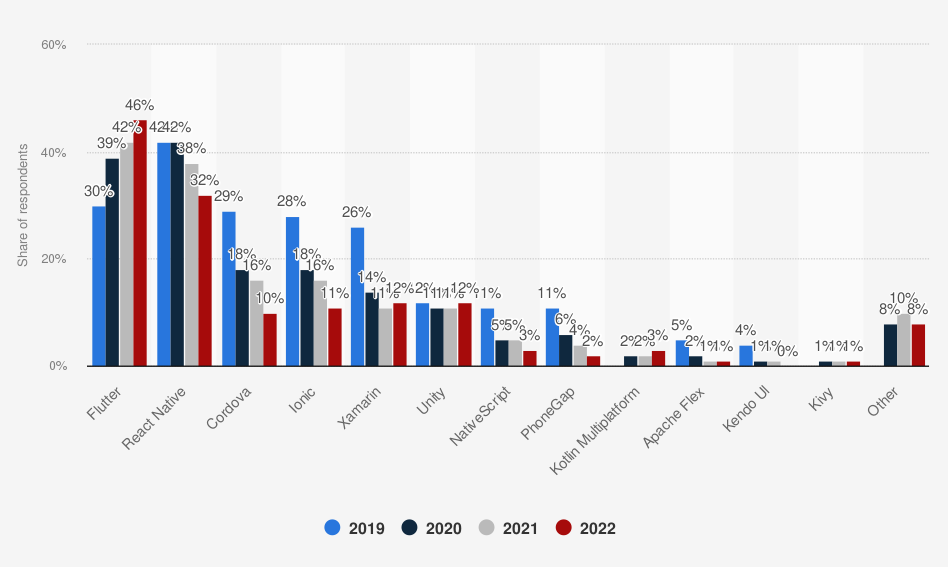
\includegraphics[scale = 0.45]{img/cross_platform-sts.png}
    \caption{Cross-platform mobile frameworks used by software developers worldwide from 2019 to 2022\cite{jetbrains2022}}
    \label{fig:cross_platform-sts}
\end{figure}
\subsubsection*{Objectives}
\begin{enumerate}
    \item To evaluate the development efficiency of Java, Kotlin, and Flutter. This includes measuring the time taken for development, the ease of implementation of features, and the integration of third-party services across the three frameworks.
    \item To analyze the maintainability of Java, Kotlin, and Flutter applications.  Maintainability will be assessed by examining code complexity, readability, and the ability to adapt or extend the application with new features.
    \item This study aims to compare the code quality of applications developed using Java, Kotlin, and Flutter. Code quality will be evaluated based on the prevalence of code smells, adherence to coding standards, and the occurrence of bugs or issues during and after development.
    \item To provide recommendations on the choice of development approach based on empirical data: Based on the findings, the study aims to offer guidelines on selecting development approaches for different mobile app projects, considering factors like project size, complexity, and specific industry needs.
\end{enumerate}
\subsubsection*{Research Questions}
In pursuit of these objectives, the study will seek to answer the following research questions:
\begin{enumerate}
    \item Comparing the Efficiency and Resource Utilization of Java, Kotlin, and Flutter: How does each technology stack up against one another regarding development efficiency, time, and resources required to create a fully operational mobile application? What are the implications of selecting each technology for the development process?
    \item Considering the Impact on Maintenance and Long-Term Code Quality: What are the consequences of choosing Java, Kotlin, or Flutter on mobile application maintainability? How do code complexity, debugging ease, and change adaptability impact long-term maintenance and code quality in these development environments?
    \item Navigating Coding Challenges and Selection Criteria: How does each development approach—Java, Kotlin, or Flutter—address prevalent coding challenges and quality issues, such as the frequency and severity of code smells? Based on these considerations, which development approach is most desirable for various mobile application projects? Considering project scope, performance requirements, and target platforms, what are the recommendations for framework selection to optimize development outcomes?
\end{enumerate}
\subsection{Methodology, Significance, and Structure of Thesis}
A robust methodology has been adopted to achieve the research objectives outlined in this study, which involves developing a Kanban board application using three distinct programming environments: Java, Kotlin, and Flutter. The subsequent analysis of these applications will employ SonarQube, a sophisticated tool designed to assess metrics such as lines of code (LOC), code smells, and overall code quality. This method not only facilitates the collection of quantitative data concerning the efficiency and maintainability of each language but also provides qualitative insights into the coding experience. Such a dual-focused analysis enables a comprehensive understanding of the practical impacts of each development approach on project outcomes.
\par
The insights derived from this research are expected to be highly valuable for developers and project managers, guiding the selection of development tools and practices based on empirical evidence. By clearly delineating the strengths and weaknesses associated with Java, Kotlin, and Flutter, this study contributes to informed decision-making within the software development community. Such knowledge is crucial for enhancing app quality and developer satisfaction, and it is anticipated that the findings will encourage more efficient and effective development practices within the industry. The practical implications of this research are significant, offering potential improvements in development processes, resource allocation, and project management in mobile app development.
\par
This thesis is methodically structured into six comprehensive chapters, designed to guide the reader through the research process systematically:

\begin{itemize}
    \item \textbf{Introduction:} This opening chapter sets the stage by outlining the motivation for the study, the research gaps identified, and the objectives to be achieved.
    \item \textbf{Literature Review:} This section delves into a thorough review of existing research, discussing the theoretical frameworks and previous empirical studies relevant to mobile application development, mainly focusing on Java, Kotlin, and Flutter.
    \item \textbf{Methodology:} This section details the specific methods employed in the study, including the development processes for the Kanban board application in each programming environment and the analytical tools and criteria used to evaluate code quality. 
    \item \textbf{Results:} This paper presents a detailed account of the application development and analysis findings, offering a comparative perspective on the code quality metrics observed across the different programming environments.
    \item \textbf{Discussion:} This section interprets the results in the context of existing literature and discusses their implications for developers and the broader software development industry.
    \item \textbf{Conclusion and Recommendations:} This section summarizes the findings, discusses the study’s potential limitations, and offers recommendations for future research and practical applications in mobile app development.
\end{itemize}

\clearpage

\section{Literature Review} \label{literature_review}
Building upon the discussion of Kotlin's integration into Android development, it is crucial to contextualize this transition by considering the origins and foundational concepts of the fundamental programming languages and frameworks in use today. To this end, we shall delve into the historical development of Kotlin, Java, and Flutter. Each of these technologies has uniquely contributed to the evolution of software development practices and choices available to mobile developers. A brief exploration of their inception and initial objectives will provide valuable insights into their current roles and capabilities within the technology landscape.
\subsection{Java}
Java was developed in 1995 by Sun Microsystems, with the initial release being Java 1.0. It was designed by James Gosling and his team as a programming language that could run on any device without recompilation, known as "write once, run anywhere" \cite{raffles1817history}. Java's structure is based on classes and objects, following the object-oriented programming paradigm. It is a statically typed language, meaning variables must be declared before they can be used, enhancing code reliability and maintainability \cite{pinto2015large}. 
\par
Java is widely used for Android app development due to its portability, security features, and extensive standard library. Android apps are primarily developed in Java, making it the de facto language for Android development \cite{li2016accessing}. The Android Software Development Kit (SDK) provides developers with tools to build apps efficiently, leveraging Java's robust features. Additionally, Java's platform independence allows Android apps to run on various devices with different hardware and software configurations, contributing to its popularity in the mobile app development industry \cite{li2016accessing}.
\par
In the context of Android, Java is utilized to access Android APIs, enabling developers to interact with the underlying operating system and create feature-rich applications \cite{li2016accessing}. The structure of Java facilitates the development of complex Android apps by providing a well-defined syntax, memory management through garbage collection, and support for multithreading, which is essential for responsive and interactive mobile applications \cite{pinto2015large}.
\subsection{Kotlin}
Kotlin, a statically typed programming language supporting object-oriented and functional programming, was developed in 2011 by JetBrains. Inspired by various languages like Groovy, Kotlin aimed to address the limitations of existing languages and provide enhanced features for developers \cite{king2020history}. Kotlin's structure is designed to be concise and expressive, offering features like improved conditional execution with the "when" structure, which allows for more optimal handling of business tasks. Additionally, Kotlin incorporates modern language features such as null-safe navigation and coroutines for asynchronous programming \cite{li2022mapping}. 
\par
Kotlin is widely used for Android app development due to its interoperability with Java, seamless integration with Android Studio, and concise syntax, which increase developer productivity \cite{li2022mapping}. The language's versatility and compatibility with existing Java codebases make it a popular choice for building Android applications. Furthermore, Kotlin's safety features, such as null safety and immutability by default, contribute to writing robust and bug-free code.
\par
In Android development, Kotlin provides developers with tools like the Kotlin Coroutines library for asynchronous programming and the Gradle Kotlin DSL for project assembly, enhancing the development process \cite{king2020history}. Its concise syntax and modern features enable developers to create efficient and maintainable Android applications \cite{kartinah2023android}. Kotlin's popularity in Android development is further evidenced by its use in various research projects focusing on Android-based applications. 
\subsection{Dart(Flutter)}
Flutter is a versatile app SDK developed by Google that allows developers to create high-performance applications for various platforms like iOS, Android, and the web using a single codebase \cite{bouchemal2020scream}. It was initially released in 2017 and has gained popularity due to its ability to provide a consistent user experience across different platforms. 
\par
Flutter's architecture is based on the Dart programming language, which Google also developed. Dart is an object-oriented, class-based language that supports interfaces, mixins, abstract classes, and optional typing. It is optimized for building user interfaces and allows for ahead-of-time compilation of native code for better performance \cite{ernawati2021android}.
\par
Flutter uses a reactive framework composed of widgets, which are the building blocks of Flutter applications. Widgets in Flutter are arranged hierarchically to create the user interface. Flutter's architecture allows for hot reload, which enables developers to see the changes they make to the code reflected in the app almost instantly, making the development process more efficient \cite{pratama2021pengembangan}.
\par
One of the critical reasons why Flutter is used is its ability to create cross-platform applications with a single codebase. This significantly reduces development time and effort as developers do not have to write separate code for different platforms. Additionally, Flutter provides a rich set of customizable widgets, a fast development cycle, and strong community support, making it an attractive choice for developers \cite{pratama2021pengembangan}.
\subsection{Previous Research}
\subsubsection*{Kotlin's Transition and Adoption in Android Development}
The transition from Java to Kotlin in Android development is motivated by Kotlin's advanced features like null safety, extension functions, and concise syntax, which collectively enhance code readability and maintainability. Kotlin's interoperability with Java and official support by Google further drive its adoption despite challenges related to the learning curve and migration efforts \cite{hegedHus2022static}. On the other hand, Flutter's emergence as a cross-platform framework offers the advantage of natively compiled applications from a single codebase across various platforms, supported by its widget-based architecture and the Dart programming language \cite{mazuera2022taxonomy}. However, concerns persist regarding Flutter's performance compared to native applications and the maturity of its ecosystem.
\par
Recent research by V. Oliveira, L. Teixeira and F. Ebert. \cite{oliveira2020adoption} explores the adoption of Kotlin for Android development through a mixed-methods approach, combining quantitative analysis of Stack Overflow discussions with qualitative interviews of Android developers. This study highlights the rapid acceptance of Kotlin following its endorsement by Google, attributing its popularity to features like null safety, expressiveness, and interoperability with Java. These attributes have facilitated a smoother transition for developers migrating from Java, enabling them to utilize existing Java libraries while benefiting from Kotlin's modern features.
\par
Developers appreciate Kotlin's concise syntax and enhanced safety features \cite{oliveira2020adoption}, contributing to more robust and maintainable code. However, the study also reveals challenges, such as the complexity introduced by Kotlin’s functional programming capabilities, which some developers find obscure and challenging to manage in larger codebases. Interoperability with Java, while largely beneficial, introduces its complexities, mainly when dealing with nullability and Java's legacy code.
\par
To determine the effect of code smells on software maintainability, Matheus Flauzino conducted an empirical analysis of the prevalence of code smells in Java and Kotlin, examining more than 6 million lines of code from 100 GitHub repositories. This paper is essential for developers debating whether to use Java or Kotlin since it shows conclusively that the latter tends to have fewer code smells, which is a surefire sign of future maintenance issues. The study analyzed five prevalent code smells and found that Kotlin consistently displays fewer examples of these troublesome patterns except for the Long Parameter List than Java. The results imply that Kotlin's design, which prioritizes readability and conciseness, may naturally prevent code smells from developing. Because of this, Flauzino et al.'s paper highlights the complex factors in selecting a programming language for software development and presents a strong case for using Kotlin over Java for projects where maintainability is a concern \cite{flauzino2018you}. 

\subsubsection*{Improving Code Quality and Software Maintenance}
The focus on code quality in mobile app development, including integrating tools like SonarQube, emphasizes the importance of managing technical debt and addressing code smells \cite{hecht2015detecting}. Innovations like ecoCode emphasize energy-efficient coding practices, reflecting a broader concern for sustainable software development. Comparative studies on development methodologies provide insights into the challenges and considerations involved in transitioning between frameworks, offering valuable practical experiences for developer \cite{lamothe2020a3}.
\par
Evaluating open-source projects offers practical insights into applying different development methodologies, aiding in identifying patterns, best practices, and common pitfalls associated with various programming languages and frameworks. Despite the wealth of knowledge on mobile app development frameworks, there is a gap in research that combines practical development experience with a thorough analysis of open-source projects across diverse frameworks, particularly in exploring the effects of methodologies on code quality metrics like code smells and their severity \cite{ardito2020effectiveness}.
\par
The prediction of code smells in continuous integration is a critical task for quality managers and developers. A recent study by Md Abdullah Al Mamun \cite{mamunimproving} investigated the effectiveness of organic versus cumulative software metrics in predicting code smells. The researchers used over 36,000 software revisions from 242 open-source Java projects to develop predictive models. Their findings revealed that non-cumulative (organic) metrics, which reflect changes between revisions rather than aggregated totals, were significantly more effective in predicting code smells. This is because organic metrics are more sensitive to recent changes in code, offering a more accurate measure for predicting software quality issues.
\par
In contrast, cumulative metrics were less effective, potentially masking recent developments that were more indicative of current software quality. The distinction between organic and cumulative metrics is essential for quality managers and developers in continuous integration environments, where quick iterations and timely quality assessments are crucial. The study also employed various model validation techniques to ensure the generalizability of the results.

\subsubsection*{Static Analysis Tools and Their Application}
Static analysis tools have been recognized as valuable for improving software quality. However, a recent study by D. Marcilio \cite{marcilio2019static} critically examined SonarQube, a leading static analysis tool, in real-world software projects across various organizational settings, including open-source communities and government institutions. The study revealed that despite the perceived effectiveness of static analysis tools in enforcing coding standards and reducing technical debt, the actual resolution rate of identified issues remains low, with an average resolution rate of only 13% across the studied projects. While problems are typically fixed within about 19 days of being reported, the low overall resolution rate suggests that many issues identified by SonarQube need to be prioritized or deemed non-critical by developers. Moreover, the customization of SonarQube instances in different organizations led to significant variance in the types of issues that are reported and addressed, with some organizations using highly customized configurations that may not effectively capture the most critical violations or could lead to a high number of false positives, further complicating the developers' decision-making process regarding which issues to address.
\par
The study conducted by Ifeanyi Rowland Onyenweaku \cite{onyenweaku2021sonarqube} aimed to evaluate the effectiveness of static analysis tools in identifying defects in software applications, with a focus on the use of SonarQube in analyzing Spectral Workbench, a tool used for capturing and analyzing spectral data. The researchers found that SonarQube successfully identified many defects, ranging from minor UI issues to critical bugs, which could cause system failures if not addressed. Their analysis revealed 232 code smells and 63 bugs, providing a detailed categorization of issues by severity and type, which could aid developers in prioritizing which issues to address first. The study also highlighted the challenge of low-resolution rates for identified issues in software development, with constraints such as prioritization, resource allocation, and perceived severity often playing a role. Despite this, the researchers emphasized the potential of integrating SonarQube into open-source projects, providing a blueprint for other projects. Overall, the findings of this study demonstrate the value of static analysis tools in enhancing the reliability and effectiveness of software applications while highlighting the challenges that need to be addressed to improve the resolution rate of identified issues.
\par
The research conducted by Sebastian Stiernborg on the application of SonarQube in the open-source project Spectral Workbench has been instrumental in providing a deeper understanding of the practical usage of this tool in a corporate setting. The study presents a comprehensive view of the operational challenges and benefits associated with implementing continuous inspection processes, thereby contributing to the body of knowledge in this domain. In his master thesis \cite{stiernborg2019automated}, Sebastian Stiernborg delves into the efficacy of implementing continuous inspection processes within software development teams, specifically focusing on SonarQube. The study was conducted in collaboration with Furhat Robotics' development team, where Stiernborg worked closely to introduce SonarQube to their existing development processes. The primary objective of the integration was to automate code reviews and improve code quality without disrupting the developers' workflow. The study presents a set of guidelines based on feedback from integrating continuous inspection tools, highlighting the advantages of such tools, including the early detection of defects and enhanced code quality. However, the study also identifies potential challenges, such as the complexity of integrating these tools within existing systems and the need for careful handling to avoid disruption and ensure developer buy-in.
\par
Furthermore, Stiernborg's research emphasizes the need for further studies to explore the integration of different continuous inspection tools and features. One of the key findings from the research is the challenge of balancing the immediate benefits of continuous inspection with the initial resistance and learning curve associated with adopting new tools. The study details the specific implementation steps taken at Furhat Robotics, including the challenges of configuring and maintaining such tools within existing systems and the strategies employed to overcome these challenges. Overall, the study contributes to the growing body of research on continuous inspection processes and highlights the importance of careful planning, implementation, and evaluation of such tools in software development teams.
\par
The study conducted by Sebastian Stiernborg \cite{stiernborg2019automated} on integrating static analysis tools and its impacts on maintenance activities was further enriched by Ze ́phyrin Soh's \cite{soh2016code} investigation. Soh's study quantified the specific effects of code smells on various maintenance tasks, offering a more detailed perspective on the implications of code quality on software maintainability. Soh's research is particularly noteworthy as it differentiates between different types of maintenance efforts, such as editing, navigating, reading, and searching, unlike previous studies that treated maintenance effort as a monolithic activity. The study revealed that code smells have varying impacts on different maintenance activities. While some code smells may increase the effort required for tasks such as navigating and editing, they do not uniformly affect all maintenance activities. For instance, the code smell "Feature Envy" significantly increased the effort required for searching activities, whereas "Data Clumps" primarily elevated the effort in editing tasks. This nuanced view provides a more granular understanding of developers' practical challenges when dealing with code smells in a maintenance context. The study also utilized a sophisticated methodological approach, utilizing multiple linear regressions to analyze the impact of code smells while considering other factors such as file size and number of revisions. This approach validates the significant role of code smells in increasing maintenance effort and refines our understanding of their impact relative to other factors such as file size and changes made.
\par
Ensuring high-quality code is fundamental to developing effective and efficient software engineering software. However, recent research \cite{corral2015better} conducted by Corral and Fronza challenges the notion that superior code quality is the primary determinant of app success in the Google Play store. The study examined the relationship between source code quality and market success indicators, such as the number of downloads and user ratings, using a sample of 100 open-source mobile applications. Results revealed a relatively marginal impact of source code quality on market success indicators, suggesting that factors such as marketing strategies, app functionality, user interface design, and overall user experience play more significant roles in determining the success of mobile applications in app stores. The methodology employed by Corral and Fronza involved using statistical methods to establish a strong correlation between established source code metrics and app store success metrics. The findings underscore the complexity of app success and highlight the limitations of relying solely on technical excellence in a market driven by consumer preferences and competitive features \cite{corral2015better}. In the research conducted by Luis Corral and Ilenia Fronza, Figure \ref*{fig:graph_lr} showcases a visual representation of the market success model based on app store metrics such as Number of Downloads (NOD), Number of Reviewers (NOR), and Application Rating (AR). This figure effectively demonstrates how these metrics collectively contribute to defining the market success of mobile applications. NOD measures the popularity and reach of an app by indicating how many times it has been downloaded, thus indirectly measuring its visibility and user interest. NOR, on the other hand, represents users' engagement with the app by counting how many users have taken the time to review it. Lastly, AR, which is averaged from all user ratings, offers a direct insight into user satisfaction and perceived app quality. Combined, these metrics provide a comprehensive view of an app's performance in the market. They portray how often it was downloaded, how well users received it, and the extent of active user interaction and satisfaction.
\begin{figure}[htbp]
    \centering
    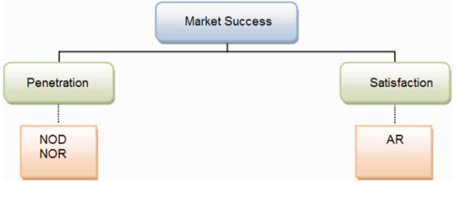
\includegraphics[scale = 0.8]{img/graph_lr.png}
    \caption{Corral and Fronza's research resulted in a Market Success Model Based on App Store Metrics.}
    \label{fig:graph_lr}
\end{figure}

The study by Michele Tufano \cite{alkhaeir2020effect} sheds light on the origins and persistence of code smells in significant software ecosystems, presenting critical insights into the internal software development processes. The empirical analysis conducted on 200 open-source projects from Android, Apache, and Eclipse ecosystems traces the history of code changes to pinpoint when specific code smells are introduced and under what conditions they are most likely to occur. The study \cite{alkhaeir2020effect} finds that many smells are introduced at the inception of code entities or through changes that do not directly relate to ongoing maintenance, challenging the prevailing assumption that code smells primarily emerge during routine maintenance and evolution activities. The research used a metric-based methodology to detect smell-induced changes, providing a granular view of how smells develop over time. The findings suggest that tool-based smell detection and refactoring recommendations should consider the specific developmental context to be truly effective and advocate for the development of more sophisticated recommendation systems that could help developers plan and implement refactoring activities more strategically, thereby potentially reducing the introduction of new smells during both development and maintenance phases.
\par
Building on Michele Tufano's analysis \cite{tufano2015and} of the origins of code smells, the research \cite{alkhaeir2020effect} conducted by Tarek Alkhaeir and Bartosz Walter sheds further light on the significant impact these smells have on the relationship between design patterns and defects. Their study \cite{alkhaeir2020effect} highlights that code smells can significantly exacerbate the likelihood of defects in software projects where design patterns are implemented. Through an analysis of Java classes from ten systems in the PROMISE dataset, Alkhaeir and Walter critically evaluate how design patterns and code smells correlate with increased defects. Their work confirms that classes utilizing design patterns are not inherently defect-prone but become so when code smells are present. The study establishes a clear connection between smelly and non-smelly design pattern classes and defects using statistical tests. The findings indicate that pattern classes with code smells experience more defects than their non-smelly counterparts, underscoring the substantial negative impact of code smells on software quality. The researchers also observed that while non-smelly design patterns tend to have a neutral or slightly negative effect on defect proneness, introducing code smells drastically increases the likelihood of defects.
\par
Xiaofeng Han and colleagues conducted a study \cite{han2021understanding} to explore the practical applications of code reviews in identifying and addressing code smells within the OpenStack community. Drawing on prior research on code smells in software systems, the study reveals that code smells are critical indicators of potential maintenance issues often overlooked during the review process. Specifically, the researchers examined code reviews within the Nova and Neutron projects and found that coding convention violations or oversights by developers were common causes of code smells. However, when code smells were identified, reviewers provided actionable recommendations for refactoring, typically implemented by developers, improving code quality.  The study highlights the value of manual code review over automated tools, as the former is more context-sensitive and effective in identifying subtle issues. The researchers found that enhancing the code review process with better guidelines and training on smell detection could further improve the effectiveness of this quality assurance practice. This collaborative approach to code review reinforces the importance of adhering to coding standards and demonstrates that code reviews are crucial to identifying and addressing code smells despite the challenges involved.




\subsubsection*{Emergence and Impact of Flutter in Cross-Platform Development}
Cross-platform development tools, including Flutter, are rapidly transforming the landscape of mobile application development by offering significant reductions in code complexity and enhancing maintainability—a study by \cite{cheon2021converting}.	Y. Cheon and C. Chavez demonstrated that when an existing Android application was rewritten in Flutter, it could run on Android and iOS platforms and required approximately 37\% fewer lines of code than the original Java implementation \cite{cheon2021converting}. This reduction is primarily attributed to Flutter's streamlined approach to UI development and robust widget library, which significantly diminishes the need for verbose UI code and extensive platform-specific adaptations.
\par
Furthermore, the transition from Java to Flutter revealed that Flutter's declarative UI framework and reactive programming model could improve application performance and responsiveness. By moving away from the imperative and stateful approaches typical in Android development, Flutter enables more dynamic and efficient handling of UI changes, leading to smoother user experiences \cite{nawrocki2021comparison} This shift is crucial for developers looking to build highly interactive and responsive applications without the overhead of managing complex state synchronization across user interface components. 
\par
The triangulation method used in the study—analyzing discourse from Stack Overflow alongside direct developer interviews—provides a comprehensive understanding of the practical challenges and benefits developers observe in real-world scenarios. This approach confirms the theoretical advantages of Kotlin discussed in previous literature and illuminates the nuanced difficulties encountered during its practical application.
\par
The evolution of programming languages like Java and Kotlin and frameworks such as Flutter has significantly shaped the landscape of Android application development. Each technology brings unique strengths for mobile app creation, from Java's "write once, run anywhere" principle to Kotlin's modern syntactic features and Flutter's cross-platform capabilities. This diversity allows developers to select technologies that best fit their project's requirements and personal or team proficiency. However, as the technology landscape continuously evolves, developers must remain adaptable, continually updating their skills and understanding of these tools. The ongoing transition towards more efficient, readable, and maintainable coding practices suggests a promising future for mobile development. By embracing these changes and learning from comparative and empirical studies, developers can better navigate the complexities of modern app development, ensuring robust, efficient, and user-friendly applications.

\clearpage

\section{Methodology}
\clearpage

% \section{Experimental Results}  \label{exp-results}
% This section focuses on the evaluation of the proposed framework, including the experimental setup, evaluation metrics, and performance results.

% \clearpage


\nocite{*}
%%%%%%%%%%%%%%%%%%%%%%%%%%%%%%%%%%%%%%%%%%%%
\bibliographystyle{unsrturl}
\bibliography{article}
\clearpage
%%%%%%%%%%%%%%%%%%%%%%%%%%%%%%%%%%%%%%%%%%%%

\appendix
\section*{Appendices}
\section{Project Listings for Automated SonarQube Analysis} \label{app:a}
\begin{table}[htbp]
	\begin{tabular}{p{5cm}|p{7cm}}
		\hline
		\cellcolor{Gray}Project Name	                                                  & \cellcolor{Gray}GitHub Link  \\ \hline
        KanbanBoardApp & \url{https://github.com/Sardor6628/Kanban-Board-Java} \\
        CountdownTimer2 & \url{https://github.com/sagarsiddhpura/CountdownTimer} \\
        Easy-Attendance-App & \url{https://github.com/jaikeerthick/Easy-Attendance-App} \\
        StopWatchRemade & \url{https://github.com/0developers/StopWatchRemade} \\
        Post-it-Notes-App & \url{https://github.com/harshkv/Post-it-Notes-App} \\
        VideoPlayer & \url{https://github.com/waleedtalha/VideoPlayer} \\
        CurrencyConverter & \url{https://github.com/Ch-Tima/CurrencyConverter/tree/master} \\
        passwordgenerator & \url{https://github.com/SecUSo/privacy-friendly-passwordgenerator} \\
        finance-manager & \url{https://github.com/SecUSo/privacy-friendly-finance-manager} \\
        todo-list & \url{https://github.com/SecUSo/privacy-friendly-todo-list} \\
        pain-diary & \url{https://github.com/SecUSo/privacy-friendly-pain-diary} \\
        qr-scanner & \url{https://github.com/SecUSo/privacy-friendly-qr-scanner} \\
        tape-measure & \url{https://github.com/SecUSo/privacy-friendly-tape-measure} \\
        pedometer & \url{https://github.com/SecUSo/privacy-friendly-pedometer} \\
        weather & \url{https://github.com/SecUSo/privacy-friendly-weather} \\
       
    \end{tabular}
	\caption{ Java Open Source Projects Selected for Analysis \label{tab:java_projects}}
\end{table}

\begin{table}[htbp]
	\begin{tabular}{p{5cm}|p{7cm}}
		\hline
		\cellcolor{Gray}Project Name	                                                  & \cellcolor{Gray}GitHub Link  \\ \hline
        KanbanBoa & \url{https://github.com/Sardor6628/Kanban-Board-Kotlin} \\
        vocable-android & \url{https://github.com/willowtreeapps/vocable-android?tab=readme-ov-file} \\
        plees-tracker & \url{https://github.com/vmiklos/plees-tracker} \\
        NotyKT & \url{https://github.com/PatilShreyas/NotyKT} \\
        muzei & \url{https://github.com/muzei/muzei} \\
        pdf-viewer-pro & \url{https://github.com/Sav22999/sav-pdf-viewer-pro} \\
        vocable & \url{https://github.com/PhilT95/ger-es_trainer} \\
        MyNotes & \url{https://github.com/akshatbhuhagal/MyNotes} \\
        RecurringExpenseTracker & \url{https://github.com/DennisBauer/RecurringExpenseTracker?tab=readme-ov-file} \\
        Simple-Dialer & \url{https://github.com/SimpleMobileTools/Simple-Dialer} \\
        PhoneBook & \url{https://github.com/KishanViramgama/PhoneBook_CRUD} \\
        SoundMeter1 & \url{https://github.com/albertopasqualetto/SoundMeterESP} \\
        Simple-Draw & \url{https://github.com/SimpleMobileTools/Simple-Draw} \\
        unitconverter & \url{https://github.com/dbrant/unitconverter-android/tree/master} \\
        Simple-Voice-Recorder & \url{https://github.com/SimpleMobileTools/Simple-Voice-Recorder/tree/master} \\
    \end{tabular}
	\caption{ Kotlin Open Source Projects Selected for Analysis \label{tab:kotlin_projects}}
\end{table}


\begin{table}[htbp]
	\begin{tabular}{p{5cm}|p{7cm}}
		\hline
		\cellcolor{Gray}Project Name	                                                  & \cellcolor{Gray}GitHub Link  \\ \hline
        KanbanBoardApp & \url{https://github.com/Sardor6628/kanban_board_crm} \\
        day-night-time-picker & \url{https://github.com/subhamayd2/day_night_time_picker.git} \\
        android-tv-app & \url{https://github.com/mawaqit/android-tv-app.git} \\
        ConsumerFlutterApp & \url{https://github.com/LaCoro/ConsumerFlutterApp.git} \\
        flutter-chat-craft & \url{https://github.com/taxze6/flutter-chat-craft.git} \\
        Flutter-TDD-Clean-Architecture-E-Commerce-App & \url{https://github.com/Sameera-Perera/Flutter-TDD-Clean-Architecture-E-Commerce-App.git} \\
        flutter-samples & \url{https://github.com/yuto-yuto/flutter_samples.git} \\
        flutter-unit & \url{https://github.com/toly1994328/FlutterUnit} \\
        flutter-quill & \url{https://github.com/singerdmx/flutter-quill.git} \\
        Musify & \url{https://github.com/gokadzev/Musify.git} \\
        Personal-Finance-Manager & \url{https://github.com/sajitha00/Personal-Finance-Manager.git} \\
        mobile & \url{https://github.com/realm/realm-dart} \\
        spotube & \url{https://github.com/KRTirtho/spotube.git} \\
        anonaddy & \url{https://github.com/KhalidWar/anonaddy} \\
        pstube & \url{https://github.com/prateekmedia/pstube.git} \\
    
    \end{tabular}
	\caption{ Dart Open Source Projects Selected for Analysis \label{tab:dart_projects}}
\end{table}

\section{Python Script for Project Automation and Configuration} \label{app:a2}

%-------------------------
\begin{lstlisting}[
	caption				= Python Scripts for Project Automation and Configuration,	% 여기에는 '_'쓸 거면 '\_'로
	label				= muapp,          % 여기에는 '_'쓸 거면  '_'로
	xleftmargin			= 4pt,
	framexleftmargin	= 4pt,
	tabsize				= 4,
	breaklines			= true,
	breakautoindent		= true,
	postbreak			= \space,
%	backgroundcolor		= \color{listingcolor}, 
	frame		= tb,
	numbers		= left,		% 이 밑으론 줄 번호 설정
	stepnumber	= 1,
	numbersep	= 1pt,
	numberstyle	= \tiny,
	escapeinside = ~~
	]	
    import subprocess
    import os
    import requests
    import base64
    def encode_credentials(username, password):
        credentials = f"{username}:{password}"
        encoded_credentials = base64.b64encode(credentials.encode()).decode()
        return encoded_credentials
    
    
    def create_sonar_project(project_key, project_name, encoded_credentials):
        url = f'http://localhost:9000/api/projects/create?project={project_key}&name={project_name}'
        headers = {
            'Authorization': f'Basic {encoded_credentials}',
            'Content-Type': 'application/x-www-form-urlencoded'
        }
        response = requests.post(url, headers=headers)
        return response
    
    
    def generate_sonar_token(project_key, token_name, encoded_credentials):
        url = f'http://localhost:9000/api/user_tokens/generate?name={token_name}&projectKey={project_key}&type=PROJECT_ANALYSIS_TOKEN'
        headers = {
            'Authorization': f'Basic {encoded_credentials}',
            'Content-Type': 'application/x-www-form-urlencoded'
        }
        response = requests.post(url, headers=headers)
        return response
    
    
    def clone_and_setup_sonar(repo_urls, save_directory, username, password):
        encoded_credentials = encode_credentials(username, password)
        os.makedirs(save_directory, exist_ok=True)
    
        for url in repo_urls:
            repo_name = url.split('/')[-1].replace('.git', '')
            clone_path = os.path.join(save_directory, repo_name)
            config_file_path = os.path.join(clone_path, 'sonarqube_configuration.txt')
            config_file_properties = os.path.join(clone_path, 'sonar-project.properties')
    
    
            # Skip cloning if repo is already cloned and configuration file exists
            if os.path.exists(clone_path) and os.path.exists(config_file_path):
                print(f'Repository "{repo_name}" already cloned and configured. Skipping...')
                continue
    
            # Clone repo if it doesn't exist
            if not os.path.exists(clone_path):
                result = subprocess.run(['git', 'clone', url, clone_path], stdout=subprocess.PIPE, stderr=subprocess.PIPE,
                                        universal_newlines=True)
                if result.returncode != 0:
                    print(f'Failed to clone {repo_name}. Error: {result.stderr}')
                    continue
    
            # Proceed with SonarQube project creation and token generation
            print(f'Cloned {repo_name}')
            project_response = create_sonar_project(repo_name, repo_name, encoded_credentials)
            if project_response.status_code == 200:
                print(f'SonarQube project created for {repo_name}')
                token_response = generate_sonar_token(repo_name, f"{repo_name}_token", encoded_credentials)
                if token_response.status_code == 200 and 'token' in token_response.json():
                    token = token_response.json()['token']
                    with open(config_file_properties, 'w') as properties_file:
                        properties_file.write(f"""
                        #Project identification
                        sonar.projectKey={repo_name}
                        sonar.projectName={repo_name}
                        sonar.projectVersion=1.0
                        
                        # Source code location.
                        # Path is relative to the sonar-project.properties file. Defaults to .
                        # Use commas to specify more than one file/folder.
                        # It is good practice to add pubspec.yaml to the sources as the analyzer
                        # may produce warnings for this file as well.
                        sonar.sources=lib,pubspec.yaml
                        sonar.tests=test
                        
                        # Encoding of the source code. Default is default system encoding.
                        sonar.sourceEncoding=UTF-8
                        """)
                    with open(config_file_path, 'w') as token_file:
                        token_file.write(f"""\n# 
                        #Project identification
                        sonar.projectKey={repo_name}
                        sonar.projectName={repo_name}
                        sonar.projectVersion=1.0
                        
                        # Source code location.
                        # Path is relative to the sonar-project.properties file. Defaults to .
                        # Use commas to specify more than one file/folder.
                        # It is good practice to add pubspec.yaml to the sources as the analyzer
                        # may produce warnings for this file as well.
                        sonar.sources=lib,pubspec.yaml
                        #sonar.tests=test
                        
                        # Encoding of the source code. Default is default system encoding.
                        sonar.sourceEncoding=UTF-8
                        
                        
                        run following:
                        
                    sonar-scanner \
      -Dsonar.projectKey={repo_name} \
      -Dsonar.sources=. \
      -Dsonar.host.url=http://localhost:9000 \
      -Dsonar.login={token}
                        
                                                 """)
    
                    print(f'SonarQube configuration saved to {config_file_path}')
                else:
                    print(f'Failed to generate SonarQube token for {repo_name}.')
            else:
                print(f'Failed to create SonarQube project for {repo_name}.')
    
        print('Finished processing repositories and setting up SonarQube projects.')
    
    
    if __name__ == '__main__':
        repo_urls = [
            #Flutter projects=
            "https://github.com/shiosyakeyakini-info/miria.git",
            "https://github.com/hoc081098/hoc081098.git",
            "https://github.com/singerdmx/flutter-quill.git"
            "https://github.com/deckerst/aves.git",
            "https://github.com/clragon/e1547.git",
            "https://github.com/PalisadoesFoundation/talawa.git",
            "https://github.com/LaCoro/ConsumerFlutterApp.git",
            "https://github.com/nank1ro/flutter-shadcn-ui",
            "https://github.com/realm/realm-dart",
            "https://github.com/KhalidWar/anonaddy",
            "https://github.com/prateekmedia/pstube.git"
        ]
        save_directory = 'flutter_repositories'
        username = 'admin'  # SonarQube username
        password = 'superadmin'  # SonarQube password
        clone_and_setup_sonar(repo_urls, save_directory, username, password)
    
\end{lstlisting}
\section{Python Script for Data Retrieval and Report Generation} \label{app:a3}

%-------------------------
\begin{lstlisting}[
	caption				= Python Script for Data Retrieval and Report Generation
	label				= muapp,          % 여기에는 '_'쓸 거면  '_'로
	xleftmargin			= 4pt,
	framexleftmargin	= 4pt,
	tabsize				= 4,
	breaklines			= true,
	breakautoindent		= true,
	postbreak			= \space,
%	backgroundcolor		= \color{listingcolor}, 
	frame		= tb,
	numbers		= left,		% 이 밑으론 줄 번호 설정
	stepnumber	= 1,
	numbersep	= 1pt,
	numberstyle	= \tiny,
	escapeinside = ~~
	]	

    import requests
import pandas as pd

pd.set_option('display.max_rows', None)  # or replace None with the exact number of rows you want
pd.set_option('display.max_columns', None)  # or replace None with the exact number of columns you want
pd.set_option('display.width', 1000)  # Adjust this number based on your display width
pd.set_option('display.max_colwidth', None)

def fetch_project_metrics_and_issues_summary(base_url, projects, types="CODE_SMELL", ps=500):
    project_summaries = []  # List to store summary data for all projects

    for project in projects:
        # Fetch issues summary
        issues_params = {
            "componentKeys": project,
            "types": types,
            "ps": ps
        }

        issues_response = requests.get(f"{base_url}/api/issues/search", params=issues_params)

        # Fetch project metrics
        metrics_params = {
            "component": project,
            "metricKeys": "ncloc,complexity,violations"
        }

        metrics_response = requests.get(f"{base_url}/api/measures/component", params=metrics_params)

        if issues_response.status_code == 200 and metrics_response.status_code == 200:
            issues_data = issues_response.json()
            metrics_data = metrics_response.json()

            # Parse issues data
            issues = issues_data.get("issues", [])
            severity_counts = {
                "BLOCKER": 0,
                "CRITICAL": 0,
                "MAJOR": 0,
                "MINOR": 0,
                "INFO": 0
            }
            for issue in issues:
                if issue["severity"] in severity_counts:
                    severity_counts[issue["severity"]] += 1

            # Parse metrics data for ncloc (Lines of Code)
            measures = metrics_data["component"]["measures"]
            loc = next((measure["value"] for measure in measures if measure["metric"] == "ncloc"), "0")

            # Prepare the summary for the current project
            project_summary = {
                "NAME": project,
                "BLOCKER": severity_counts["BLOCKER"],
                "CRITICAL": severity_counts["CRITICAL"],
                "MAJOR": severity_counts["MAJOR"],
                "MINOR": severity_counts["MINOR"],
                "INFO": severity_counts["INFO"],
                "total": len(issues),
                "LOC": loc  # Add LOC to the project summary
            }

            project_summaries.append(project_summary)
        else:
            print(
                f"Failed to fetch data for project {project}, issues status code: {issues_response.status_code}, metrics status code: {metrics_response.status_code}")

    return pd.DataFrame(project_summaries)


# Example usage
base_url = "http://localhost:9000"
projects = ["Kanban_board_flutter","day_night_time_picker", "android-tv-app", "ConsumerFlutterApp", "flutter-chat-craft",
            "Flutter-TDD-Clean-Architecture-E-Commerce-App", "flutter_samples", "Kanban_board_flutter", "flutter-quill",
            "Musify", "openfoodfacts-dart", "Personal-Finance-Manager",
            "mobile", "spotube", "anonaddy", "pstube"]
project_metrics_and_issues_summary_df = fetch_project_metrics_and_issues_summary(base_url, projects)
# Display the table
print(project_metrics_and_issues_summary_df)

# Save the DataFrame to a CSV file
report_path = "flutter-report.csv"
project_metrics_and_issues_summary_df.to_csv(report_path, index=False)
print(f"Flutter Report saved to {report_path}")

projects = ["Kanban_board_java", 'CountdownTimer2', '2048-android2', 'Easy-Attendance-App', 'StopWatchRemade',
            'Post-it-Notes-App', 'VideoPlayer', 'CurrencyConverter', 'passwordgenerator', 'finance-manager',
            'todo-list', 'pain-diary', 'qr-scanner', 'tape-measure', 'pedometer', 'weather']

project_metrics_and_issues_summary_df = fetch_project_metrics_and_issues_summary(base_url, projects)
# Display the table
print(project_metrics_and_issues_summary_df)

# Save the DataFrame to a CSV file
report_path = "java-report.csv"
project_metrics_and_issues_summary_df.to_csv(report_path, index=False)
print(f"Java Report saved to {report_path}")

projects = ["Kanban_board_kotlin", "vocable-android", "plees-tracker", "NotyKT",
            "muzei", "awaker", "GitExplorer-Android",
            'pdf-viewer-pro', 'vocable', 'MyNotes',
            'RecurringExpenseTracker',
            'Simple-Dialer', 'PhoneBook',
            'SoundMeter1', 'Simple-Draw', 'unitconverter', 'Simple-Voice-Recorder']

project_metrics_and_issues_summary_df = fetch_project_metrics_and_issues_summary(base_url, projects)
# Display the table
print(project_metrics_and_issues_summary_df)

# Save the DataFrame to a CSV file
report_path = "kotlin-report.csv"
project_metrics_and_issues_summary_df.to_csv(report_path, index=False)
print(f"Kotlin Report saved to {report_path}")

\end{lstlisting}



\section{Implementation Details of Task Models}\label{app:TaskResponse}
\begin{lstlisting}[
	caption				= Java Task Model Implementation,	
	label				= javaModel,         
	xleftmargin			= 20pt,
	framexleftmargin	= 20pt,
	tabsize				= 4,
	breaklines			= true,
	breakautoindent		= true,
	postbreak			= \space,
	frame		= tb,
	numbers		= left,		% 이 밑으론 줄 번호 설정
	stepnumber	= 1,
	numbersep	= 5pt,
	numberstyle	= \tiny,
	escapeinside = ~~
	]%--------------------여기부터 코드(한 줄 Enter 필수)
		

    package com.example.kanban_board_java.data.response;
    import com.google.firebase.firestore.Exclude;
    public class TaskResponse {
        private String id;
        @Exclude
        private String documentId;
        private String title;
        private String userId;
        private String description;
        private Long createdTime;
        private Long completedTime;
        private Long startedTime;
        private long spentTime;
        private String currentStatus;
        public String getId() {
            return id;
        }
        public void setId(String id) {
            this.id = id;
        }
        public String getDocumentId() {
            return documentId;
        }
        public void setDocumentId(String documentId) {
            this.documentId = documentId;
        }
        public String getTitle() {
            return title;
        }
        public void setTitle(String title) {
            this.title = title;
        }
        public String getUserId() {
            return userId;
        }
        public void setUserId(String userId) {
            this.userId = userId;
        }
        public String getDescription() {
            return description;
        }
        public void setDescription(String description) {
            this.description = description;
        }
        public Long getCreatedTime() {
            if (createdTime == null) {
                return 1000L;
            }
            return createdTime;
        }
        public void setCreatedTime(Long createdTime) {
            this.createdTime = createdTime;
        }
        public Long getCompletedTime() {
            if (completedTime == null) {
                return 1000L;
            }
            return completedTime;
        }
        public void setCompletedTime(Long completedTime) {
            this.completedTime = completedTime;
        }
        public Long getStartedTime() {
            if (startedTime == null) {
                return 1000L;
            }
            return startedTime;
        }
        public void setStartedTime(Long startedTime) {
            this.startedTime = startedTime;
        }
        public long getSpentTime() {
            return spentTime;
        }
        public void setSpentTime(long spentTime) {
            this.spentTime = spentTime;
        }
        public String getCurrentStatus() {
            return currentStatus;
        }
        public void setCurrentStatus(String currentStatus) {
            this.currentStatus = currentStatus;
        }
    }    
\end{lstlisting}

\begin{lstlisting}[
	caption				= Kotlin Task Model Implementation,	
	label				= kotlinModel,         
	xleftmargin			= 20pt,
	framexleftmargin	= 20pt,
	tabsize				= 4,
	breaklines			= true,
	breakautoindent		= true,
	postbreak			= \space,
	frame		= tb,
	numbers		= left,		% 이 밑으론 줄 번호 설정
	stepnumber	= 1,
	numbersep	= 5pt,
	numberstyle	= \tiny,
	escapeinside = ~~
	]
    package com.example.kanban_board_java_kotlin.data.response
import android.os.Parcelable
import com.google.firebase.firestore.Exclude
import kotlinx.parcelize.Parcelize
@Parcelize
data class TaskResponse(
    var id: String = System.currentTimeMillis().toString(),
    @get:Exclude var documentId: String = "",
    var title: String = "",
    var userId: String = "",
    var description: String = "",
    var createdTime: Long? = null,
    var completedTime: Long? = null,
    var startedTime: Long? = null,
    var spentTime: Long = 0,
    var currentStatus: String = "todo"
) : Parcelable
\end{lstlisting}

\begin{lstlisting}[
	caption				= Dart Task Model Implementation,	
	label				= dartModel,         
	xleftmargin			= 20pt,
	framexleftmargin	= 20pt,
	tabsize				= 4,
	breaklines			= true,
	breakautoindent		= true,
	postbreak			= \space,
	frame		= tb,
	numbers		= left,		% 이 밑으론 줄 번호 설정
	stepnumber	= 1,
	numbersep	= 5pt,
	numberstyle	= \tiny,
	escapeinside = ~~
	]
    import 'package:kanban_board/constants/contant_variables.dart';
    class Task {
      final String id;
      final String title;
      final String userId;
      final String description;
      final DateTime? createdTime;
      final DateTime? completedTime;
      final DateTime? startedTime;
      final int spentTime;
      final String currentStatus;
      Task({
        required this.id,
        required this.title,
        required this.userId,
        required this.description,
        required this.createdTime,
        required this.completedTime,
        required this.startedTime,
        required this.spentTime,
        required this.currentStatus,
      });
      factory Task.fromFirestore(Map<String, dynamic> data, String id) {
        return Task(
          id: id,
          title: data['title'],
          userId: data['userId'],
          description: data['description'],
          createdTime: data['createdTime'] != null
              ? DateTime.fromMicrosecondsSinceEpoch(data['createdTime'])
              : null,
          completedTime: data['completedTime'] != null
              ? DateTime.fromMicrosecondsSinceEpoch(data['completedTime'])
              : null,
          startedTime: data['startedTime'] != null
              ? DateTime.fromMicrosecondsSinceEpoch(data['startedTime'])
              : DateTime.now(),
          spentTime: data['spentTime'] != null ? data['spentTime'] : 0,
          currentStatus: data['currentStatus'],
        );
      }
\end{lstlisting}

\clearpage

\clearpage

\begin{eabstract}
환치기는 전통적이고 비공식적인 자금 이전 시스템으로, 자금세탁과 같은 목적으로 전 세계 여러 지역에서 널리 사용되고 있다. 금융 기관들이 취한 규제 조치에도 불구하고, 환치기는 여전히 테러 자금 조달 계획에서 주요한 노드이다. 그리고 그의 남용 정도는 알려지지 않았다. 환치기의 은닉 거래와 제한된 지식으로 인해 각 국가의 법적 단속기관들은 환치기를 감지하고 규제하기 어렵다. 본 논문은 그래프 마이닝 기법을 사용하여 금융 거래 데이터의 흐름에서 잠재적인 환치기 사례를 탐지하기 위한 새로운 접근 방법을 제시한다. 환치기의 특성을 반영하기 위해 제안된 프레임워크는 중심성과 이상 탐지와 같은 그래프 신경망을 이용한 그래프 마이닝 방법을 채택한다. 실험 결과, 제안된 방법은 환치기를 탐지하는 데 의미 있는 결과를 제공하며 기존 거래 모니터링 트랙에 보완적인 도구로 사용될 수 있음을 보여준다.	
\end{eabstract}

%\newpage
%\begin{thankpage}
%\input{thesis/thanks}
%\end{thankpage}

\end{document}